\section{Image Segmentation}

% Image segmentation and types
Image segmentation is a well-known problem in Computer Vision, where an image is divided into several parts (segments) to serve a purpose.

There are other types of segmentation. In our scope, we opted for semantic segmentation models for our watermark detection task in our watermark removal pipeline. For example, in Figure \ref{figure:sam-all}, Segment Anything model \cite{kirillov2023segment} return segmented pixels belonging to available classes.

We selected semantic segmentation instead of detection, because the segmented result fits the object, rather than returns a bounding box.

\begin{figure}[ht]
    \centering
    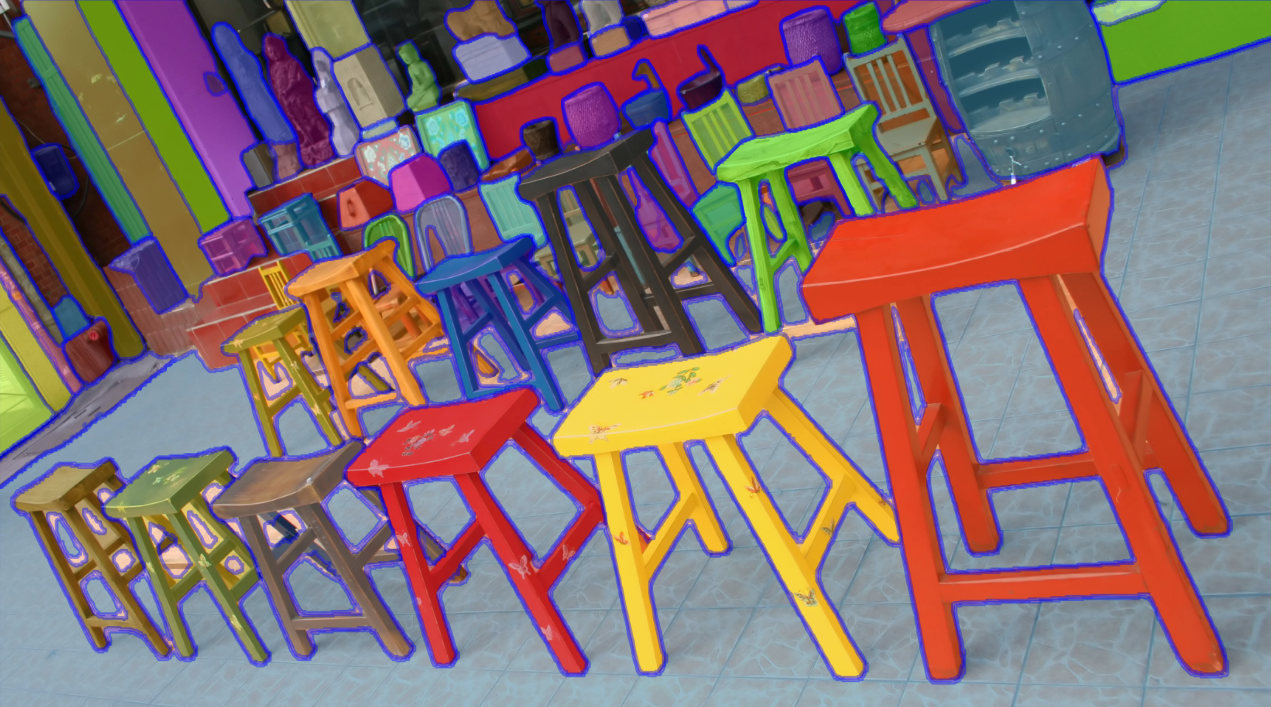
\includegraphics[width=0.8\textwidth]{img/sam-segmented-all.png}
    % 
    \caption[An image segments returned by SAM]{An image segments returned by SAM \cite{kirillov2023segment}}
    \label{figure:sam-all}
\end{figure}

% Why chosen
% In our proposed pipeline, we firstly segment an image to predict the region occupied by the watermark. Especially, Semantic segmentation suffices for our needs as it simply entails predicting which pixels are probable components of a watermark, but no further specific instances. 

% If using detection, we have to train another model to detect watermarks of a given training set, and hope that the model can generalize to unseen watermarks. Meanwhile, the watermark in an image will automatically be segmented out as it does not belong to any available class.


% There are commonly three types of segmentation. Regional segmentation divides an image into several constituent regions, usually based on the correlation between pixels in the image. Semantic segmentation classifies each pixel to one of aforementioned classes, or assigns to each pixel a distribution on the classes. This second type of segmentation is a generalization of classification. Instance segmentation goes beyond semantic segmentation, that it also detects difference instances of the same class in an image.





